\documentclass[titlepage]{article}
\usepackage[left=15mm,right=15mm,top=1in,bottom=1in]{geometry}
\usepackage{framed}
\usepackage{caption}
\usepackage{imakeidx}
\usepackage{graphicx}
\usepackage{hyperref}
\usepackage{array}
\usepackage{amsmath}

\newcolumntype{C}[1]{>{\centering\arraybackslash}m{#1cm}}
\graphicspath{{./img/}}

\makeindex

\title{\textbf{\Huge{Offer Acceptance Prediction Tool}}\\[20mm]Advanced Optimization Laboratory\\~\\\textbf{\Huge{Low-Level Software Design}}}
\author{Eric Le Fort}
 
\begin{document}
\maketitle
\tableofcontents
~\\[15mm]
\listoftables
\listoffigures


\vfill
\begin{table}[!htbp]
\centering
\begin{tabular}{| C{3}| C{2}| C{10} |}\hline
	Date			&Revision \#	&Comments\\\hline
	23-JUN-2017		&0				&- Initial document creation\\\hline
	04-NOV-2017		&1				&- Updated to reflect current state of software.\\\hline
\end{tabular}
\caption{Revision History}
\label{tab:RevisionHistory}
\end{table}
\newpage
 
\section{Introduction}
This document's purpose is to describe the low-level design of the software which will predict the likelihood of an applicant accepting an offer of enrolment. It will provide strong enough detail to guide initial development as well as future efforts to modify this system.
\subsection{Overview}
This document has four sections not including this one. Each section contains either design diagrams or in-depth explanation to further describe the architecture of this system.\\
\begin{itemize}
	\item \textbf{Program Diagrams:}This section will provide a detailed class diagram, analysis class diagram, and use case diagram for this system. The detailed class diagram will provide a breakdown of the contents of each class as well as the connections between various classes. The analysis class diagrams will define the various classes in each program in more detail, including the nature of the flow of data between them and their type (boundary, controller, or entity). The use case diagram will provide an insight into the flow of how this system handles its various uses.
	\item \textbf{Task Handling:}This section will define how the program will handle various tasks. First, it will define the protocols used for data and request communication. Then it will describe the scheduling of tasks by providing timing constraints for various operations. Next it will identify potential errors as well as plans on how to deal with those errors. Lastly, it will provide any necessary sequence diagrams in order to illustrate its use cases.
	\item \textbf{Class Responsibility Collaboration (CRC) Cards:}This section will break the program into its classes. Responsibilities of each class as well as any collaboration required (if any) with other classes to fulfill each responsibility will be defined.
	\item \textbf{Module Guide:}This section will outline the responsibilities, secrets, Module Interface Specification (MIS), and Module Interface Design (MID) of each module. It will also provide a state chart for each module to illustrate its flow.
\end{itemize}
\subsection{Naming Conventions \& Definitions}
This section is meant to outline the various definitions, acronyms and abbreviations that will be used throughout this document in order to familiarize the reader prior to reading. All necessary acronyms, abbreviations, definitions and anything of that nature can be found in the \textit{Requirements}document for this module.
\newpage



\section{Program Diagrams}
The following section will contain diagrams which will provide a preliminary overview of the system's construction.
\subsection{Detailed Class Diagram}
This diagram depicts the full system broken down by classes including relationships between those classes, the data stored in those classes, and the methods of those classes.\\[10mm]
\begin{center}
	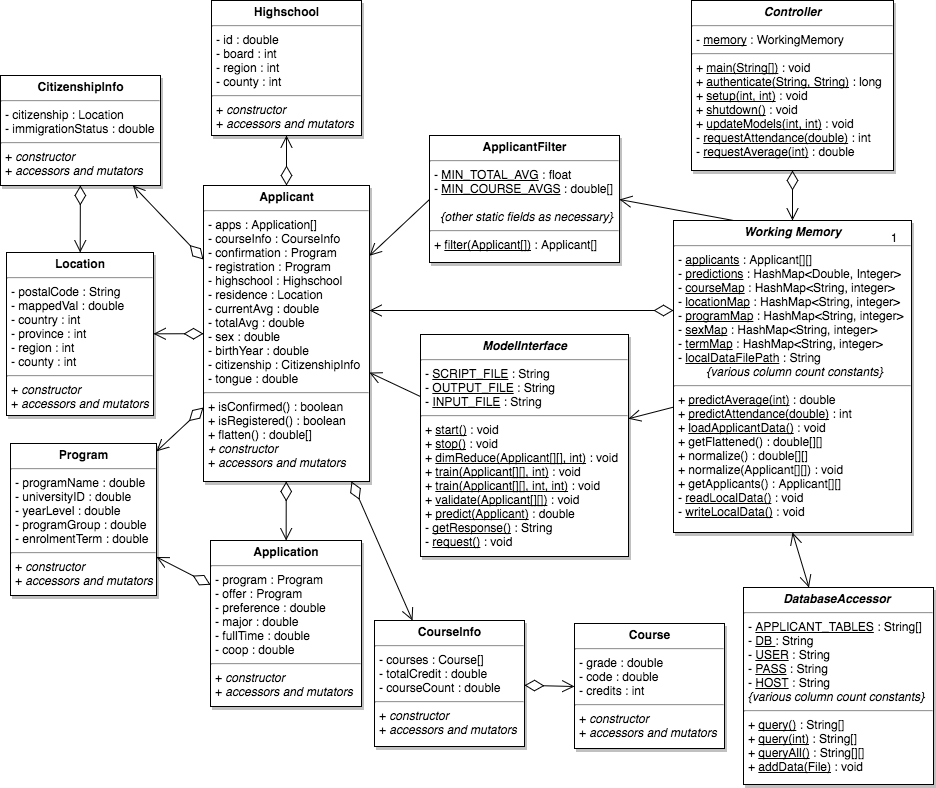
\includegraphics[width=1.05\textwidth]{AdvolDetailedClassDiagram.png}
\captionof{figure}{Detailed Class Diagram}
\label{fig:detailed class diagram}
\end{center}
\newpage
\subsection{Analysis Class Diagram}
This diagram depicts all the classes and their interactions. The arrows' directions are meant to depict the flow of data between them.\\[10mm]
\begin{center}
	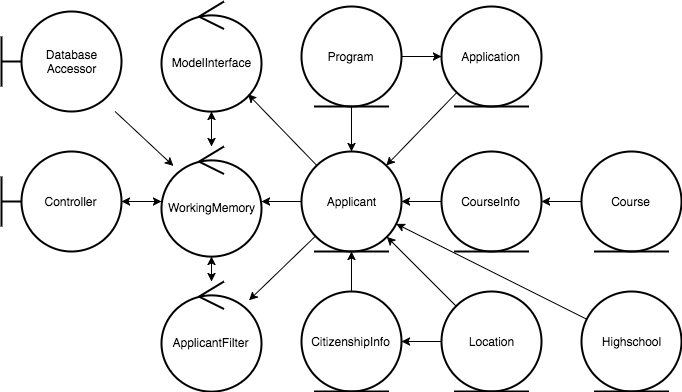
\includegraphics[width=\textwidth]{AdvolAnalysisClassDiagram.png}
\captionof{figure}{Analysis Class Diagram}
\label{fig:analysis class diagram}
\end{center}
\newpage
\subsection{Use Case Diagram}
This diagram will depict how the various use cases for this module will be handled.
\begin{center}
	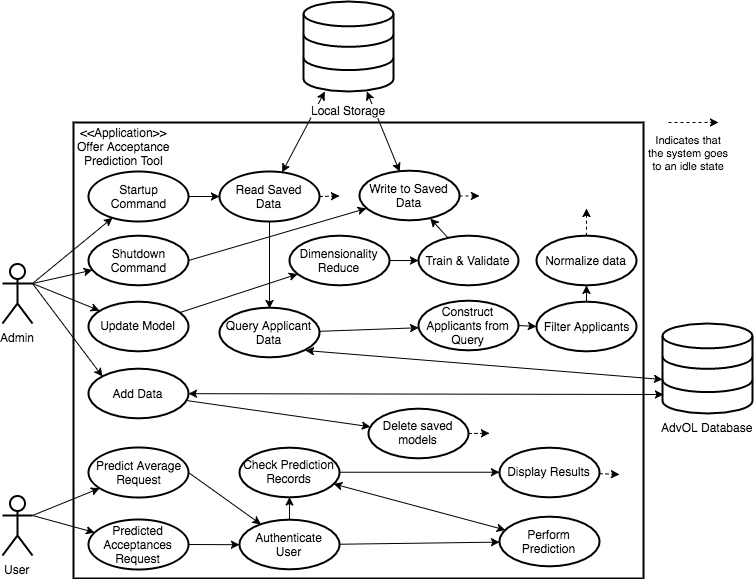
\includegraphics[width=\textwidth]{AdvolUseCaseDiagram.png}
\captionof{figure}{Use Case Diagram}
\label{fig:use case diagram}
\end{center}



\section{Task Handling}
The following section will describe how this system will perform its tasks.
\subsection{Data and Request Protocols}
Data entry will occur three times per year: once upon receiving initial applicant data, once upon receiving finalized applicant data, and once upon receiving the results of registration. Therefore it is feasible to perform manual data entry.\\~\\
The main requests to this system include acceptance grade prediction requests and attendance prediction requests.\\~\\
While handling these requests, the system must verify that the user has been authenticated. This will be achieved by firstly performing user authentication. Once the user is authenticated, their security token can be used to verify their identity during future data transfer. All network traffic will also be encrypted as an added layer of security.

\subsection{Scheduling of Tasks}
Task scheduling will not be a large area of concern for this project. Model training will occur when new data is available but that will not occur frequently. It is likely that most or even all predictions can be performed in its idle state (prior to when the user will need to access the system). In the case that a user makes a request while an idle prediction is being made, that process will be terminated prematurely. Furthermore, since there will be such a low volume of users, load testing will not be much of a concern either.
\subsection{Error Handling}
While training, an operator should be available to deal with errors that arise. This will include automated tests to verify that the model is returning reasonable results. Note that these tests should use data that is strictly separate from that used in the process of model training.\\~\\
If an error arises during use, the error should be logged and the user will be presented with a message informing them of the error. If the error persists, the user should contact the administrator of the system or a support engineer as necessary.
\subsection{Sequence Diagrams}
These sequence diagrams will depict the sequence of events for each use case.
\begin{center}
	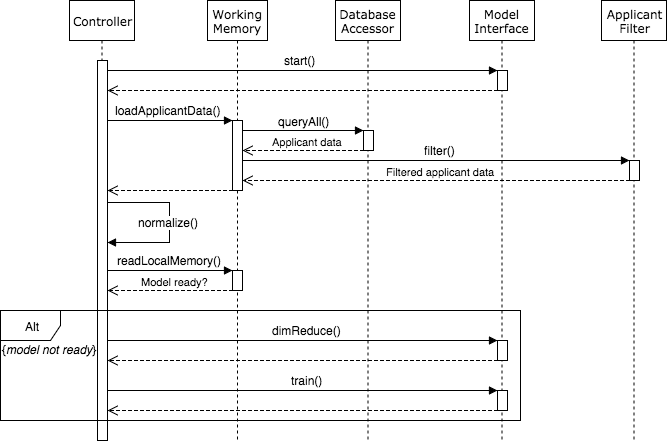
\includegraphics[width=\textwidth]{AdvolStartupSequenceDiagram.png}
\captionof{figure}{Startup Sequence Diagram}
\label{fig:startup sequence diagram}
\end{center}
\begin{center}
	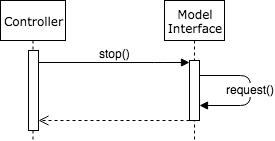
\includegraphics[width=0.4\textwidth]{AdvolShutdownSequenceDiagram.png}
\captionof{figure}{Shutdown Sequence Diagram}
\label{fig:shutdown sequence diagram}
\end{center}%~\vfill
\begin{center}
	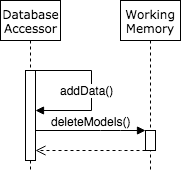
\includegraphics[width=0.27\textwidth]{AdvolAddDataSequenceDiagram.png}
\captionof{figure}{Add Data Sequence Diagram}
\label{fig:add data sequence diagram}
\end{center}
\begin{center}
	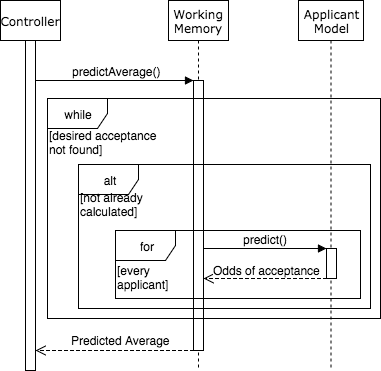
\includegraphics[width=0.6\textwidth]{AdvolPredictAverageSequenceDiagram.png}
\captionof{figure}{Predict Average Sequence Diagram}
\label{fig:predict average sequence diagram}
\end{center}
\begin{center}
	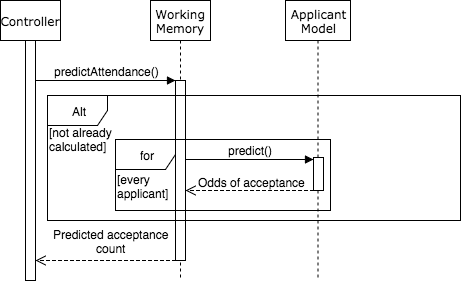
\includegraphics[width=0.75\textwidth]{AdvolPredictAcceptanceSequenceDiagram.png}
\captionof{figure}{Predict Acceptance Sequence Diagram}
\label{fig:predict acceptance sequence diagram}
\end{center}



\section{Module Guide}
This section discusses the various modules that this system is comprised of. The responsibilities, secrets, MIS, and MID will be discussed for each module.

\subsection{Controller}
\textbf{Responsibilities}
\begin{itemize}
	\item[-] User Authentication
	\item[-] Initializing necessary procedures for training, dimensionality reduction, startup/shutdown, and performing predictions
\end{itemize}~\\
\textbf{Secrets}
\begin{itemize}
	\item[-] The authentication protocol
\end{itemize}~\\
\textbf{MIS}\\[2mm]
This module is an always-running process which handles interfacing with the GUI as well as authenticating user access to the system. This module also regulates control flow through the rest of the system. Its ``inputs'' are requests from the GUI and its outputs are the authentication token or the result of a prediction.\\[6mm]
\newpage
\noindent\textbf{MID}\\[2mm]
The state chart below provides a succinct depiction of this module's internal design.\\
\begin{center}
	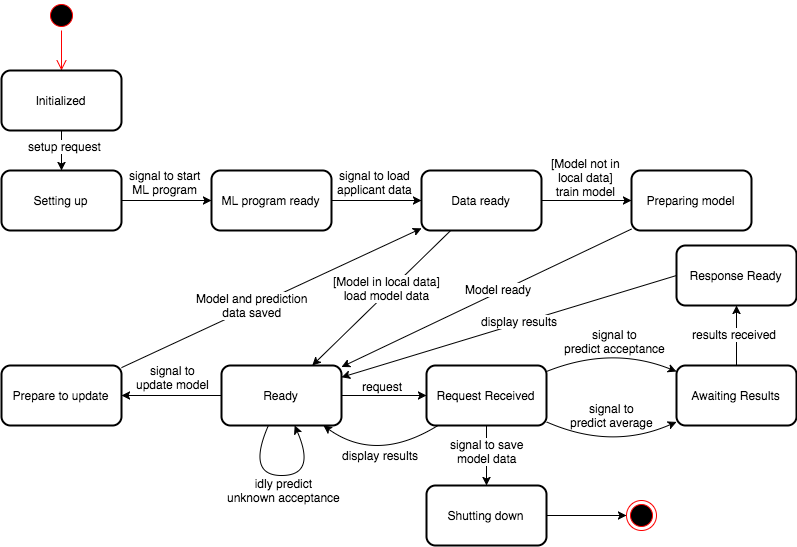
\includegraphics[width=0.9\textwidth]{AdvolControllerStateChart.png}
\captionof{figure}{Controller State Chart}
\label{fig:controller state chart}
\end{center}~\\

\subsection{DatabaseAccessor}
\textbf{Responsibilities}
\begin{itemize}
	\item[-] Querying the database for applicant records
	\item[-] Adding new applicant records to the database
\end{itemize}~\\
\textbf{Secrets}
\begin{itemize}
	\item[-] The method of querying the database
	\item[-] The method of adding new data to the database
\end{itemize}~\\
\newpage
\noindent\textbf{MIS}\\[2mm]
This module handles all database operations for the system. In particular, it provides the ability to safely query the database or insert new rows into the database. The ``inputs'' to this module are the requests and the outputs are the results of the query or nothing (if performing an insertion operation).\\[6mm]
\textbf{MID}\\[2mm]
This module acts as a boundary between the database and the rest of the system. After receiving an input String, it will build and clean the query to prevent undesired database actions. Once prepared, this submodule will query the database and return the results as a 2-dimensional array of Strings.\\[6mm]

\subsection{ApplicantFilter}
\textbf{Responsibilities}
\begin{itemize}
	\item[-] Filtering the list of applicants to impose hard limits
\end{itemize}~\\
\textbf{Secrets}
\begin{itemize}
	\item[-] The filtering parameters and values
\end{itemize}~\\
\textbf{MIS}\\[2mm]
This module handles filtering an array of applicants according to certain parameter thresholds (e.g. minimum averages for certain courses). Its input is an array of applicants and its output is a subset of the array passed in.\\[6mm]
\textbf{MID}\\[2mm]
This module's operation will be simple. It will receive an array of applicants, apply its filtering rules to remove applicants that do not satisfy its conditions, and then return that filtered list.\\[6mm]

\subsection{ModelInterface}
\textbf{Responsibilities}
\begin{itemize}
	\item[-] Initializing the machine learning program
	\item[-] Interfacing with the machine learning program
	\item[-] Sending the termination signal to the machine learning program
\end{itemize}~\\
\textbf{Secrets}
\begin{itemize}
	\item[-] The method of communicating with the machine learning program
\end{itemize}~\\
\newpage
\noindent\textbf{MIS}\\[2mm]
This module handles interfacing with the machine learning program (the \textit{Machine Learning Program} module) by passing along requests from the \textit{Controller}. Inputs to this module include the set of all applicant data, the data of a single applicant, and the desired number of clusters (for certain algorithms). The only output from this module is the likelihood that a certain applicant accepts an offer.\\[6mm]
\textbf{MID}\\[2mm]
This interface will handle sending applicant data to and receiving results from another process (that may be in a different language entirely). Two sockets, an input and an output, will be created to funnel the data between processes. Readers will clear their socket after they are finished reading the message. Writers must wait for a ``clean'' socket before writing their message. Further, this interface will also handle starting and stopping the other process. Starting will simply involve executing a bash command and stopping just involves sending a termination message to the other process.\\~\\
The state chart below depicts this module's internal design.\\
\begin{center}
	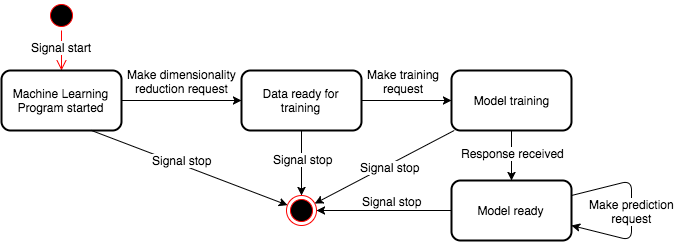
\includegraphics[width=0.8\textwidth]{AdvolModelInterfaceStateChart.png}
\captionof{figure}{ModelInterface State Chart}
\label{fig:modelinterface state chart}
\end{center}~\\

\subsection{Machine Learning Program}
\textbf{Responsibilities}
\begin{itemize}
	\item[-] Predicting the likelihood of an applicant accepting an offer
\end{itemize}~\\
\textbf{Secrets}
\begin{itemize}
	\item[-] The algorithm used
	\item[-] The specific structure and other hyper-parameters of the model
	\item[-] The weightings which define the model
\end{itemize}~\\
\textbf{MIS}\\[2mm]
This module handles training models, storing the weightings and structure associated with the trained models, and reloading previously trained models upon request. This module will facilitate using a trained model to predict the likelihood that a given applicant will accept an offer of admission. The input for this module will be the set of features for an applicant and the output will be a probability between 0 and 1.\\[6mm]
\textbf{MID}\\[2mm]
This module will be able to perform several different operations.\\~\\
One operation this module must be able to perform is training models using a set of applicant data and the results of those applications. This module will receive specifications of what sort of algorithm to use for both training and dimensionality reduction. All information will be provided using the input socket defined in the specification of the \hbox{\textit{ModelInterface}} module. During training, the model will be saved once certain accuracy checkpoints are hit. Once training is complete, a response will be sent back to the \textit{ModelInterface} using the output socket.\\~\\
Another operation this module must be able to perform is loading a specified model into memory that has been previously trained. This will be received as a request from the \textit{ModelInterface} as well as the type and location of the model to be loaded. This module will then load the appropriate type of model into memory.\\~\\
The last operation this module must be able to perform is using the model loaded into memory to perform a prediction on an applicant. The \textit{ModelInterface} will specify the type of request, the dimensionality reduction technique to use, and provide the applicant's data. That data will then be transformed using the specified dimensionality reduction technique and fed into the model. The resulting percentage will then be sent back to the \textit{ModelInterface} using the output socket.\\[6mm]

\subsection{WorkingMemory}
\textbf{Responsibilities}
\begin{itemize}
	\item[-] Store system data such as applicants and their data
	\item[-] Fetch data from other members of the system (e.g. requesting the \textit{DatabaseAccessor} retrieve applicant data)
	\item[-] Reading from and writing to local storage
\end{itemize}~\\
\textbf{Secrets}
\begin{itemize}
	\item[-] The procedure for loading applicant data
	\item[-] The method of reading and writing data to storage
	\item[-] The normalization method
	\item[-] The method of computing the predicted acceptances
	\item[-] The method of computing the predicted acceptance average
\end{itemize}~\\
\textbf{MIS}\\[2mm]
This module will handle constructing and consolidating applicant data in memory for the prediction system. To this end, it will build objects from raw String data results of database queries, normalize data, and store and retrieve prediction results. This module will store the trained applicant models and array of applicants.\newpage
\noindent\textbf{MID}\\[2mm]
Some of the functionality of this module is straightforward. The loading of applicant data is as simple as building objects from a formatted String. Normalization will just use elementary statistical methods to set an average of 0 and a standard deviation of 1.\\~\\
One of the more intricate tasks will be saving and reading data. This will occur whenever the system shuts down or before a model update occurs and will involve writing data to and reading data from a file. Models will be saved in subfolders along with the results of their previous predictions and some metadata including structure and performance information.\\~\\
Another of the more intricate tasks is predicting the attendance for a certain acceptance average. This will involve first checking to see if the prediction has been previously performed. If it has been, it will return the previous result. Otherwise, it will initialize the process of performing the necessary prediction.\\~\\
The last task is of predicting an acceptance average for a particular preferred enrolment count. This will involve doing a line search of predictions for various attendances. This will work since a larger acceptance average will always result in a projected attendance that is equal to or greater than lower acceptance averages.\\~\\
The state chart below depicts this module's internal design.\\
\begin{center}
	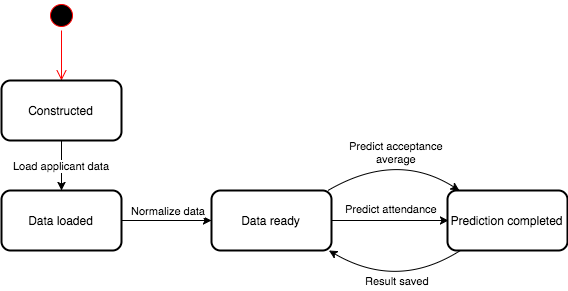
\includegraphics[width=0.75\textwidth]{AdvolWorkingMemoryStateChart.png}
\captionof{figure}{WorkingMemory State Chart}
\label{fig:workingmemory state chart}
\end{center}~\\

\newpage
\subsection{Applicant, Application, CitizenshipInfo, CourseInfo, Courses, HighSchool, Program}
\textbf{Responsibilities}
\begin{itemize}
	\item[-] Storing all data relevant to applicants
\end{itemize}~\\
\textbf{Secrets}\\[2mm]
\indent None.\\[6mm]
\textbf{MIS}\\[2mm]
These classes store all applicant data and provide access to that data.\\[6mm]
\textbf{MID}\\[2mm]
These modules are simple enough not to necessitate internal design specifications.
\end{document}




